\documentclass[11pt]{article}

% Change "review" to "final" to generate the final (sometimes called camera-ready) version.
% Change to "preprint" to generate a non-anonymous version with page numbers.
\usepackage[]{acl}
\usepackage{times}
\usepackage{latexsym}

% For proper rendering and hyphenation of words containing Latin characters (including in bib files)
\usepackage[T1]{fontenc}
% For Vietnamese characters
% \usepackage[T5]{fontenc}
% See https://www.latex-project.org/help/documentation/encguide.pdf for other character sets

% This assumes your files are encoded as UTF8
\usepackage[utf8]{inputenc}
\usepackage{microtype}
\usepackage{inconsolata}
\usepackage{graphicx}
\usepackage{listings}
\usepackage{float}

% If the title and author information does not fit in the area allocated, uncomment the following
%
%\setlength\titlebox{<dim>}
%
% and set <dim> to something 5cm or larger.

\title{Group 14 Progress Report:\\Phishing Email Detection}


\author{Virochaan Ravichandran Gowri, Hamza Abou Jaib, Mohammad Mahdi Mahboob, Omar Al-Asfar \\
  \texttt{\{ravicv3,aboujaih,mahbom2,alasfaro\}@mcmaster.ca} }

%\author{
%  \textbf{First Author\textsuperscript{1}},
%  \textbf{Second Author\textsuperscript{1,2}},
%  \textbf{Third T. Author\textsuperscript{1}},
%  \textbf{Fourth Author\textsuperscript{1}},
%\\
%  \textbf{Fifth Author\textsuperscript{1,2}},
%  \textbf{Sixth Author\textsuperscript{1}},
%  \textbf{Seventh Author\textsuperscript{1}},
%  \textbf{Eighth Author \textsuperscript{1,2,3,4}},
%\\
%  \textbf{Ninth Author\textsuperscript{1}},
%  \textbf{Tenth Author\textsuperscript{1}},
%  \textbf{Eleventh E. Author\textsuperscript{1,2,3,4,5}},
%  \textbf{Twelfth Author\textsuperscript{1}},
%\\
%  \textbf{Thirteenth Author\textsuperscript{3}},
%  \textbf{Fourteenth F. Author\textsuperscript{2,4}},
%  \textbf{Fifteenth Author\textsuperscript{1}},
%  \textbf{Sixteenth Author\textsuperscript{1}},
%\\
%  \textbf{Seventeenth S. Author\textsuperscript{4,5}},
%  \textbf{Eighteenth Author\textsuperscript{3,4}},
%  \textbf{Nineteenth N. Author\textsuperscript{2,5}},
%  \textbf{Twentieth Author\textsuperscript{1}}
%\\
%\\
%  \textsuperscript{1}Affiliation 1,
%  \textsuperscript{2}Affiliation 2,
%  \textsuperscript{3}Affiliation 3,
%  \textsuperscript{4}Affiliation 4,
%  \textsuperscript{5}Affiliation 5
%\\
%  \small{
%    \textbf{Correspondence:} \href{mailto:email@domain}{email@domain}
%  }
%}

\begin{document}
\maketitle
% \begin{abstract}
% \end{abstract}

\section{Introduction}


Phishing emails remain a prevalent and costly cybersecurity threat. They cost organizations billions of dollars annually and frequently lead to large-scale data breaches and identity theft \citep{Almomani2013}. These fraudulent messages are designed to deceive recipients into giving up sensitive information, such as passwords, bank credentials, or personal data, often by mimicking legitimate communications from trusted entities. While modern spam filters successfully intercept many obvious threats, sophisticated phishing attempts often closely imitate the language and formatting of genuine emails, allowing them to evade traditional rule-based detection systems.

The goal of this project is to develop a Natural Language Processing (NLP) classifier capable of accurately distinguishing phishing emails from legitimate ones. By framing the problem as a binary text classification task, an additional layer of automated protection can be developed to help reduce the success rate of phishing attacks. Several challenges inherently make this task difficult: phishing emails often employ language that closely mirrors legitimate business correspondence, the linguistic strategies used by attackers evolve continuously to evade existing filters, and class imbalance is a recurring concern because phishing emails are typically far less common than legitimate emails in real-world environments. Prior work has shown that both manual feature engineering \citep{Fette2007} and learning from pre-trained language models \citep{Devlin2019} are effective approaches to this problem.

To address these challenges, a balanced dataset was curated from well-known public email corpora \citep{Champa2024}. This dataset was used to explore both traditional machine learning approaches, such as Bag-of-Words with Logistic Regression, and modern transformer-based models. The classifiers were evaluated using the F1-score as the primary metric, supplemented by accuracy, precision, and recall, to ensure a robust assessment of phishing detection performance.

\section{Related Work}

Phishing email detection has been studied extensively in both the cybersecurity and NLP communities. \citet{Almomani2013} provide a comprehensive survey of phishing email filtering techniques, categorizing approaches into list-based, heuristic, visual-similarity, and machine-learning methods. They highlight that content-based machine learning classifiers consistently outperform static rule sets as phishing tactics evolve.

Early machine learning work by \citet{Fette2007} demonstrated that a Random Forest classifier trained on hand-crafted features, including the presence of URLs, the structure of embedded links, and the use of JavaScript, could identify phishing emails with over 96\% accuracy. In a complementary study, \citet{AbuNimeh2007} compared Logistic Regression, Support Vector Machines, Bayesian Additive Regression Trees, and Neural Networks on a bag-of-words representation of email text. They found that no single algorithm dominated across all evaluation metrics and that the quality of the feature representation was at least as important as the model selection itself.

\citet{Basnet2008} explored an expanded feature set that combined textual cues with structural email properties, such as sender domain and header anomalies. This approach achieved strong results with an SVM classifier and reinforced the value of metadata-aware models.

More recently, deep learning techniques have advanced the state of the art. \citet{Alhogail2021} proposed a Graph Convolutional Network applied to email body text, reaching approximately 98\% accuracy and showing that representation-learning methods can capture subtle semantic patterns that traditional feature engineering misses. The success of pre-trained language models such as BERT \citep{Devlin2019} has significantly impacted the field. Fine-tuned transformer models have been shown to exceed a 95\% F1-score on phishing benchmarks by leveraging contextual word embeddings that capture the nuanced phrasing characteristic of social-engineering attacks.


This project draws on insights from both traditional and neural approaches. The curated phishing email corpus released by \citet{Champa2024} was utilized, which aggregates data from the TREC, SpamAssassin, and CEAS corpora. The subsequent experiments evaluate Bag-of-Words baselines alongside fine-tuned transformer architectures to identify the most effective strategy for the balanced dataset.

\section{Dataset}

\subsection{Overview}
The dataset used for this project is a curated subset of the Figshare ``Seven Phishing Email Datasets'' \citep{Champa2024}, a large repository of publicly available email corpora compiled for phishing detection research. This subset draws from five individual datasets within the repository: TREC-5, TREC-6, TREC-7, CEAS-08, and SpamAssassin. These sources were selected because they contain rich email metadata, including sender address, receiver address, subject line, and a binary URL flag, in addition to the raw email body, providing a realistic representation of the features that real-world email filters would evaluate.

\subsection{Data Collection and Balancing}
To construct a balanced dataset, 1,500 phishing and 1,500 legitimate entries were extracted from each of the five sub-datasets, yielding a total of 15,000 data points with a perfect 50/50 class distribution. This design prevents any single source corpus from dominating the training signal and ensures sufficient data points from both classes. During collection, rows with missing or incomplete fields were skipped; because the original repository is sufficiently large, omitting these entries did not compromise the target sample size. Data collection proceeded by filtering on the provided label column and selecting entries sequentially until 1,500 valid data points per class were obtained from each sub-dataset. The final dataset was assembled on February~19,~2026.

\subsection{Dataset Format}
The data is stored as a single CSV file in which each row represents one email. The columns are summarized in Table~\ref{tab:dataset-format}.

\begin{table}[h]
\centering
\small
\begin{tabular}{lll}
\hline
\textbf{Column} & \textbf{Description} & \textbf{Type} \\
\hline
Sender   & Email address of the sender    & Text \\
Receiver & Email address of the recipient & Text \\
Date     & Timestamp of the email         & Text \\
Subject  & Subject line text              & Text \\
Body     & Body content text              & Text \\
Label    & Ground-truth class             & Binary \\
Urls     & Whether the email contains URLs & Binary \\
\hline
\end{tabular}
\caption{Dataset schema. The \texttt{Label} column is coded as 0 (legitimate) or 1 (phishing); the \texttt{Urls} column is coded as 0 (no URLs) or 1 (contains URLs).}
\label{tab:dataset-format}
\end{table}

\subsection{Preprocessing}
Minimal preprocessing was applied to the raw data. HTML tags were stripped from the email body field so that classifiers operate on linguistic content rather than markup code. Date formats were standardized to a more human-readable format to ensure consistency and ease of understanding during the annotation phase. No additional stop-word removal, stemming, or lemmatization was performed at the dataset level; such transformations were instead applied within individual model pipelines to allow fair comparison across different feature-extraction strategies.

\subsection{Annotation and Agreement}
Although the dataset includes pre-existing labels from the original corpora, a secondary annotation pass was conducted to verify label quality and familiarize the evaluation team with the underlying data. The first 480 samples of the dataset were selected for annotation and split equally among four annotators. The annotators then swapped sections and independently re-labeled the first 40 samples of their new partition, producing 160 double-annotated instances. Each sample took approximately 45~seconds to annotate. Inter-annotator agreement was measured using Cohen's Kappa on the 160 double-annotated data points, yielding $\kappa = 0.9$, indicating excellent agreement. This high agreement is partly attributable to the technical background of the team, which made it easier to successfully recognize common phishing indicators such as suspicious URLs, urgent language, and impersonated sender-domains.

\subsection{Dataset Partitioning}
The 15,000-instance corpus was partitioned into three non-overlapping subsets to support rigorous evaluation and mitigate overfitting: a training set comprising 70\% of the data (10,500~emails), a validation set comprising 15\% (2,250~emails) for hyperparameter tuning, and a held-out test set comprising the remaining 15\% (2,250~emails) whose labels are withheld during development.

\subsection{Sensitive Content Disclaimer}
Because the dataset contains real-world emails from public archives, evaluators and potential users may encounter content related to financial fraud, fake legal threats, and adult-oriented spam. Some emails may also contain personally identifiable information such as names, email addresses, and phone numbers of individuals. All data is used strictly for research and classification purposes in compliance with the terms of service of the Figshare platform.

\section{Features}

The models implemented in this project vary significantly in their approach to feature representation to compare differing strategies. Model 1 utilizes static, manually created feature pipelines composed of TF-IDF sparse vectors supplemented by engineered numeric metadata. In contrast, Models 3 and 4 forgo explicit feature engineering entirely and instead rely on the dynamic, contextual word embeddings produced by pre-trained Transformer architectures, which are learned as part of the model during fine-tuning. This variation allows for a direct comparison between an interpretable, engineered feature pipelines versus end-to-end representation learning.

\subsection{Model 1: RoBERTa and TF-IDF Ensemble}
To capture both semantic meaning and structural metadata, a single text input was created for each email by concatenating the sender's domain, the subject line, and the email body. The subject line was included twice in this string to increase its weighting in the text representation, which makes sense because subjects often contain the strongest and most immediate indicators of phishing attempts (such as false urgency or administrative threats).

Two distinct feature representations were used to vary the experiments. For the Logistic Regression branch, the text was transformed using TF-IDF on both word n-grams (unigrams to trigrams) and character n-grams (3 to 5 characters). This static sparse representation captures specific phrases and unusual spellings. In addition to the text features, seven numeric features were engineered: the character lengths of the subject and body, the counts of URLs, exclamation marks, dollar signs, a count of urgent keywords (such as ``password'', ``suspended'', and ``verify''), and a binary flag for the presence of URLs. These features were explicitly added because phishing heavily relies on malicious links, aggressive exclamation formatting, and fabricated urgency to deceive users. For the Transformer branch, rather than static representations, the model utilized dynamic contextual word embeddings. The engineered text was encoded using the \texttt{roberta-base} tokenizer, and the embeddings were learned entirely as part of the model, specifically truncated to a maximum length of 512 tokens. Feature selection was also naturally performed, as the TF-IDF vocabulary was capped at the most frequent 80,000 word and 30,000 character n-grams.

\subsection{Model 2: Random Forest Classifier}
The text input concatenates the subject and body fields, which are tokenized through lowercasing, removal of punctuation and stop-words, and Porter stemming. Initially, these tokens were vectorized using \texttt{CountVectorizer}, but this was subsequently replaced with \texttt{TfidfVectorizer}. This TF-IDF weighting reduces the influence of common, uninformative tokens, while the inclusion of bigrams captures characteristic phishing phrases (such as "click here") that unigrams cannot account for.

A second set of 13 manual features was taken from the email details ignored by the first model. These include URL counts, subject and body length, capitalization ratios, exclamation mark and dollar sign usage, an urgency word count, and a flag for free email domains (like Gmail). These numeric features were joined with the TF-IDF text data using the \texttt{hstack} function from the \texttt{scipy} library to form the final input for the classifier.

\subsection{Model 3: RoBERTa-Base}
Because this approach utilizes a fine-tuned architecture, representation learning was prioritized to take full advantage of the pretrained attention transformer. To effectively utilize this capacity, the text input was formatted as follows:

\begin{lstlisting}[
  caption={Input format for the RoBERTa model.},
  label={lst:rob_input_format}
]
[SUBJECT] <{Subject content}>
[BODY] <{Body content}>
[SENDER] <{Sender content}>
\end{lstlisting}

This structured format allowed RoBERTa's contextualized embeddings to distinctly separate \textit{subject}, \textit{body}, and \textit{sender} information during processing. The specific concatenation order was chosen so that the primary email contents were prioritized during tokenization prior to the sender identity. This ordering helps prevent legitimate but infrequent communicators from being incorrectly flagged as phishing.

\subsection{Model 4: ELECTRA Base}
Similarly, because ELECTRA is a fine-tuned architecture, representation learning was prioritized to leverage the pretrained attention transformer. To utilize this capacity natively, the text input was formatted as follows:

\begin{lstlisting}[
  caption={Input format for the ELECTRA model.},
  label={lst:elc_input_format}
]
[SENDER] <{Sender content}>
[SUBJECT] <{Subject content}>
[BODY] <{Body content}>
\end{lstlisting}

This layout allowed ELECTRA's contextualized embeddings to distinctly separate \textit{sender}, \textit{subject}, and \textit{body} information. The specific order was selected because it mirrors the natural flow of information in a standard email. Furthermore, because ELECTRA operates as a discriminative model, providing the sender identity first allows it to aggressively prioritize address identification when determining if an email originates from a phishing source.

\section{Implementation}

All models were evaluated against shared baselines provided by the Codabench benchmark: a naive majority vote classifier (which always predicts the most frequent class) and a baseline Logistic Regression trained on standard Bag-of-Words features. All implemented models successfully outperformed the naive baseline. Furthermore, Model 1 implements an internal ablation study by running its two components (Logistic Regression and RoBERTa) as standalone classifiers prior to ensemble blending, revealing the independent contribution of each feature set.

\subsection{Model 1: RoBERTa and TF-IDF Ensemble}
This implementation uses a probability-based ensemble approach that combines a traditional machine learning classifier with a fine-tuned Transformer. Several versions of the model were run independently on the data, effectively serving as an ablation study to see how each standalone framework performed before the ensemble blending.

The first component is a Logistic Regression model trained on the combined TF-IDF and numeric features. The model was trained to minimize the log-loss (cross-entropy) using the L-BFGS optimization technique, with the regularization parameter set to $C=5.0$. 

The second component is a \texttt{roberta-base} sequence classification model. Optimization was performed using AdamW to minimize the standard cross-entropy loss function. This model was fine-tuned for 5 epochs with a batch size of 16, a learning rate of $1 \times 10^{-5}$ with a 15\% warmup ratio, and a weight decay of 0.01. The best model checkpoint was saved based on the validation F1-score.

The final classifier blends the predicted probabilities from both models. By testing different blend weights on the validation set, an optimal alpha of 0.55 was found, meaning RoBERTa's prediction contributed slightly more (55\%) than the Logistic Regression (45\%) to the final output. The classification threshold was also tuned from the default 0.5 to 0.46, maximizing the overall F1-score.

\subsection{Model 2: Random Forest Classifier}
This model was implemented using the \texttt{RandomForestClassifier} from the \texttt{scikit-learn} library. Trees were grown using the Gini impurity metric, which minimizes the probability of mislabeling a random sample at each node split. As an ensemble of decision trees, there is no gradient-based loss function for this implementation. Various hyperparameter combinations were evaluated, resulting in a final configuration utilizing 500 decision trees, balanced class weights (\texttt{class\_weight='balanced'}), and a \texttt{max\_features} cap of 500. Because the default maximum feature parameter is too low relative to the dimensionality of the large TF-IDF vocabulary, raising this threshold increased the likelihood of finding meaningful signals at each node split.

Finally, similar to Model 1, the \texttt{predict\_proba} function was utilized to expose raw classification probabilities. The decision threshold was tuned iteratively on the validation set, selecting the boundary between 0.30 and 0.70 that maximized the final F1-score. This strategy ensured that the entire pipeline was formally optimized against the validation F1-score rather than raw accuracy. Overall, the pipeline combines TF-IDF bigram text features, custom input features, and a tuned Random Forest into a single lightweight classifier that requires no GPU and remains fully interpretable via feature importances.

\subsection{Model 3: RoBERTa-Base}
The RoBERTa-Base model was fine-tuned for binary classification through several processing steps. The pretrained \texttt{roberta-base} checkpoint was loaded via \texttt{AutoModelForSequenceClassification} with 2 labels. The corresponding tokenizer was used to encode all inputs with maximum-length padding and truncation to 512 tokens, representing the maximum context window supported by the architecture.

Training was performed using the \texttt{Trainer} API from the \texttt{transformers} package. The following hyperparameters were utilized: a learning rate of $2 \times 10^{-5}$, a weight decay of 0.01, and a per-device batch size of 8 with gradient accumulation over 4 steps, yielding an effective batch size of 32. Mixed-precision training (\texttt{fp16}) was enabled, and the model was fine-tuned for 5 epochs. Model checkpoints were saved after each epoch, and the best checkpoint was automatically restored at the end of training based on the validation F1-score. The standard cross-entropy loss supplied internally by the \texttt{Trainer} API was minimized using the AdamW optimizer.

\subsection{Model 4: ELECTRA Base}
\texttt{google/electra-base-discriminator} was fine-tuned for binary sequence classification using the Hugging~Face \texttt{transformers} library. The pretrained checkpoint was loaded via \texttt{AutoModelForSequenceClassification} with \texttt{num\_labels=2}, and the corresponding tokenizer was used to encode all inputs with maximum-length padding and truncation.

Training was performed using the \texttt{Trainer} API with the following hyperparameters: a learning rate of $5 \times 10^{-5}$, a per-device batch size of 8 with gradient accumulation over 4 steps (yielding an effective batch size of 32), mixed-precision training (\texttt{fp16=True}), weight decay of 0.01, and 3 training epochs. The model was evaluated every 100 steps on the validation set, and the best checkpoint was automatically restored at the end of training based on the validation F1-score. The loss function used was the standard cross-entropy loss, minimized using the AdamW optimizer as provided by the Hugging~Face Trainer API.

\section{Results and Evaluation}

\subsection{Evaluation Strategy}
The evaluation strategy partitioned the data into a 70\% training split (10,500 samples), a 15\% validation split (2,250 samples), and a 15\% held-out test split (2,250 samples). To prevent label bias, the class distributions were maintained at a perfectly balanced 50/50 split between phishing and legitimate emails across all dataset partitions. The F1-score was used as the primary evaluation metric because it provides a reliable and unskewed balance between precision and recall. In the context of phishing detection, both metric extremes carry severe consequences: low precision (high false positives) results in legitimate, potentially critical emails being wrongfully filtered into a spam folder, while low recall (high false negatives) allows dangerous security threats to reach the user's inbox. Therefore, optimizing for the harmonic mean via the F1-score ensures that a model does not aggressively sacrifice one constraint for the other. Accuracy, precision, and recall were also tracked to provide a comprehensive assessment across all implementations.

\subsection{Results}
For comparison, two general baselines were provided by the Codabench benchmark dataset:
\begin{itemize}
    \item \textbf{Majority Vote Baseline:} F1 = 0.6667, Accuracy = 0.5000, Precision = 0.5000, Recall = 1.0000.
    \item \textbf{Logistic Regression with Bag-of-Words (Benchmark):} F1 = 0.8196, Accuracy = 0.8116, Precision = 0.7861, Recall = 0.8560.
\end{itemize}

\subsubsection{Model 1: RoBERTa and TF-IDF Ensemble}
Final test evaluations were obtained by submitting the model's predictions to the Codabench evaluation system. On the test set, the ensemble model achieved an F1-score of 0.9844, an accuracy of 0.9844, a precision of 0.9884, and a recall of 0.9804. This demonstrates that the model successfully generalizes to unseen data, effortlessly outperforming both the provided majority vote baseline and the primary test benchmark.

\subsubsection{Model 2: Random Forest Classifier}

As shown in Table~\ref{tab:rf-results}, incorporating TF-IDF bigrams and explicitly engineered metadata (V2) improved both the F1-score and accuracy over the initial Bag-of-Words implementation (V1). The final iteration (V3) introduced decision threshold tuning and restricted the architecture to a maximum of 500 features per split. This shifted the precision-recall trade-off significantly: recall increased substantially while precision dropped, indicating that the optimized threshold caused the model to predict phishing with greater aggression. Comparing all versions indicates that the model has reached a general performance bottleneck; further hyperparameter tuning merely transfers performance penalties between different evaluation metrics rather than consistently eliminating errors. Continuing to increase parameters, such as the total decision tree count, or introducing additional features would likely increase computational complexity without yielding proportional gains. Nonetheless, all three iterations comfortably outperform both Codabench baselines and serve as exceptionally lightweight implementations compared to the fine-tuned transformer alternatives.

\begin{table}[h!]
\centering
\scriptsize
\begin{tabular}{lcccc}
\hline
\textbf{Version} & \textbf{F1} & \textbf{Acc.} & \textbf{Prec.} & \textbf{Rec.} \\
\hline
V1 (BoW)      & 0.9539 & 0.9542 & 0.9604 & 0.9476 \\
V2 (TF-IDF + feats.)   & 0.9603 & 0.9604 & 0.9633 & 0.9573 \\
V3 (tuned + threshold) & 0.9593 & 0.9587 & 0.9448 & 0.9742 \\
\hline
\end{tabular}
\caption{Random Forest test results across model versions.}
\label{tab:rf-results}
\end{table}

\subsubsection{Model 3: RoBERTa Base}
Final test evaluations were obtained by submitting the model's predictions to the Codabench evaluation system. On the test set, the fine-tuned RoBERTa-Base model achieved an F1-score of 0.9853, an accuracy of 0.9853, a precision of 0.9875, and a recall of 0.9831. These results demonstrate that the model successfully generalizes to unseen data, significantly outperforming both the majority vote baseline and the primary test benchmark.

\subsubsection{Model 4: ELECTRA Base}
Final test evaluations were obtained by submitting the model's predictions to the Codabench evaluation system. On the test set, the fine-tuned ELECTRA model achieved an F1-score of 0.9848, an accuracy of 0.9849, a precision of 0.9884, and a recall of 0.9813. These results demonstrate that the model generalizes effectively to unseen data, comfortably surpassing both the majority vote baseline and the Logistic Regression with Bag-of-Words benchmark provided by the dataset.

\subsection{Comparison to Peer Implementations}
To contextualize the results against alternative approaches, the implemented models were compared with those developed by other teams in the course (Table~\ref{tab:results-comparison}). Because the Codabench evaluation system only accepts raw CSV files containing predicted labels, the exact hyperparameters, preprocessing steps, and source code of these peer implementations were entirely obscured. Consequently, only their general model architectures and final evaluation metrics could be recorded for comparison. 

As shown in Table~\ref{tab:results-comparison}, all fine-tuned transformer models from both this project and peer implementations performed similarly well, tightly clustering around an F1-score of 0.98. This indicates a ceiling effect where standard transformer fine-tuning comprehensively solves the majority of the dataset, leaving only highly disguised edge cases as errors. 

When comparing specific architectures, the peer \texttt{bert-base-uncased} model achieved the highest overall precision (0.9937), demonstrating an extremely conservative posture against false positives. However, the implemented RoBERTa-Base model (Model 3) matched its overall performance by establishing a slightly stronger balance with recall, securing the highest aggregate F1-score across all implementations (0.9853). Furthermore, the peer validation of \texttt{distilbert-base} proved that lightweight, distilled transformers can achieve outstanding performance (F1 = 0.9807) without the heavy computational footprint of full-base networks like ELECTRA or RoBERTa. Interestingly, the \texttt{deberta-v3-small} peer implementation evaluated slightly lower (F1 = 0.9687), narrowing the performance gap enough to validate that strategically engineered traditional classifiers (such as Model 2's Random Forest) can remain highly competitive with structurally reduced transformer variants. Finally, the zero-shot baseline (\texttt{bart-large-mnli}) performed exceptionally poorly with an F1-score of 0.3595, cementing the conclusion that domain-specific fine-tuning is strictly required to solve this phishing classification task.

\begin{table*}[h]
\centering
\small
\begin{tabular}{l c c c c}
\hline
\textbf{Model} & \textbf{F1} & \textbf{Accuracy} & \textbf{Precision} & \textbf{Recall} \\
\hline
\multicolumn{5}{c}{\textit{Baselines}} \\
\hline
Majority Vote                      & 0.6667 & 0.5000 & 0.5000 & 1.0000 \\
LR with BoW                        & 0.8196 & 0.8116 & 0.7861 & 0.8560 \\
\hline
\multicolumn{5}{c}{\textit{Project Implementations}} \\
\hline
Model 1: Ensemble (RoBERTa + TF-IDF) & 0.9844 & 0.9844 & 0.9884 & 0.9804 \\
Model 2: Random Forest Classifier       & 0.9603 & 0.9604 & 0.9633 & 0.9573 \\
Model 3: RoBERTa Base              & 0.9853 & 0.9853 & 0.9875 & 0.9831 \\
Model 4: ELECTRA Base              & 0.9848 & 0.9849 & 0.9884 & 0.9813 \\
\hline
\multicolumn{5}{c}{\textit{Peer Implementations}} \\
\hline
\texttt{bert-base-uncased} (Fine-tuned)       & 0.9852 & 0.9853 & 0.9937 & 0.9769 \\
\texttt{distilbert-base} (Fine-tuned)         & 0.9807 & 0.9809 & 0.9892 & 0.9724 \\
\texttt{deberta-v3-small} (Fine-tuned)        & 0.9687 & 0.9693 & 0.9879 & 0.9502 \\
\texttt{bart-large-mnli} (Zero-shot)          & 0.3595 & 0.5391 & 0.5891 & 0.2587 \\
\hline
\end{tabular}
\caption{Comparison of project implementations against general baselines and peer approaches.}
\label{tab:results-comparison}
\end{table*}

\section{Error Analysis}

By systematically examining the evaluation metrics across the test dataset, we evaluated the predominant error modes of the implemented models. Comparing Model 1 (Ensemble), Model 3 (RoBERTa), and Model 4 (ELECTRA) reveals highly similar performance profiles. All three models achieve high precision scores (ranging from 0.9875 to 0.9884) while exhibiting a very slight gap in recall (ranging from 0.9804 to 0.9831). This indicates that the performance of the models differs only marginally; they are highly aggressive at minimizing false positives but share a common weakness in false negatives.

\subsection{Model 1: RoBERTa and TF-IDF Ensemble}
Systematic examination of the evaluation metrics reveals distinct patterns in the errors the model makes. Specifically, the metrics show that the model is extremely good at classifying legitimate emails accurately without falsely flagging them, as indicated by the high precision (0.9884) and the minimal false positives depicted in Figure~\ref{fig:model1-confmatrix}. It rarely produces false positives, which is critical for establishing real-world trust in a spam filter where missing important emails is highly disruptive.

However, the slightly lower recall (0.9804) indicates that the model is comparatively worse at catching highly disguised threats, resulting in more false negatives. When comparing the performance of the components, the errors predominantly occur when sophisticated phishing attempts completely omit obvious spam keywords and mimic casual conversational tones well. Because the model relies substantially on engineered text patterns, these emails fail to trigger the classifier. To specifically address these issues in future iterations, we recommend integrating external reputation-checking systems, such as automated URL domain cross-referencing or sender authentication parsing, rather than relying exclusively on the text content.

\begin{figure}[h]
  \centering
  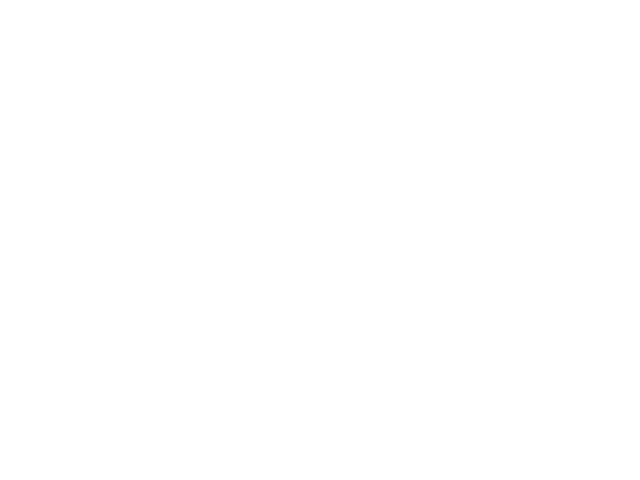
\includegraphics[width=\columnwidth]{Images/ensemble_cfm.png}
  \caption{Model 1 Confusion Matrix}
  \label{fig:model1-confmatrix}
\end{figure}

\subsection{Model 2: Random Forest Classifier}
Error analysis reveals that this model predominantly fails on complex phishing emails that successfully simulate legitimate conversational language and avoid explicit trigger terms. In these cases, the TF-IDF representation struggles due to an inherent lack of sequential context. Conversely, legitimate emails containing financial terminology or urgent language (such as IT verification notices) frequently trigger false positives, which can be visualized in the corresponding confusion matrix (Figure~\ref{fig:model2-confmatrix}). The model also struggles with aggressively concise messages containing isolated links, as the sparse feature space fails to trigger broader token matching.

Despite these limitations, the model is highly reliable on conventional phishing formats that utilize common phrasing. Unlike the transformer architectures, the Random Forest model relies heavily on explicit token presence to determine feature importance. Given the minimal degradation in accuracy compared to the deeply fine-tuned architectures, the implemented features appear highly sufficient for this task, proving that computationally expensive context-learning is not strictly required to achieve strong baseline spam filtering.

\begin{figure}[h]
  \centering
  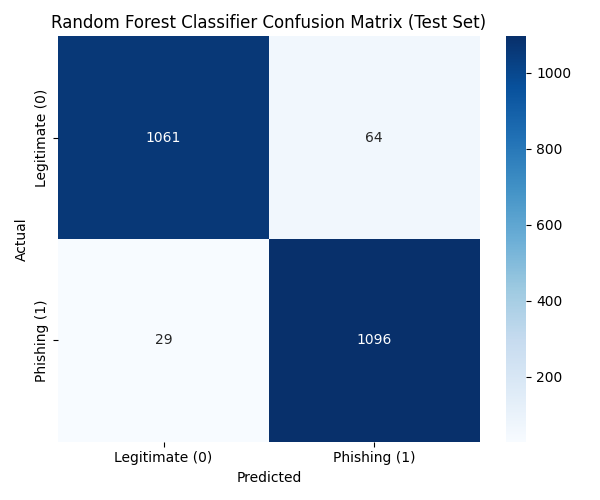
\includegraphics[width=\columnwidth]{Images/rfclf_cfm.png}
  \caption{Model 2 Confusion Matrix}
  \label{fig:model2-confmatrix}
\end{figure}

\subsection{Model 3: RoBERTa Base}
The RoBERTa model performed robustly across all evaluation metrics. Consistent with the other models, precision and recall were both exceptionally high, though the model was marginally more likely to predict phishing emails as legitimate (false negatives), as seen in the attached confusion matrix (Figure~\ref{fig:model3-confmatrix}). This mirrors the error distribution observed in Model 1, indicating that neither the TF-IDF ensemble nor the standalone RoBERTa architecture fully resolved this weakness. 

The causes of these errors may be tied to the architectural constraint of a 512-token maximum sequence length, causing the model to lose context on exceedingly long email chains. Conversely, the model could also struggle with extremely concise phishing vectors that lack sufficient structural context to trigger a detection mechanism.

\begin{figure}[h]
  \centering
  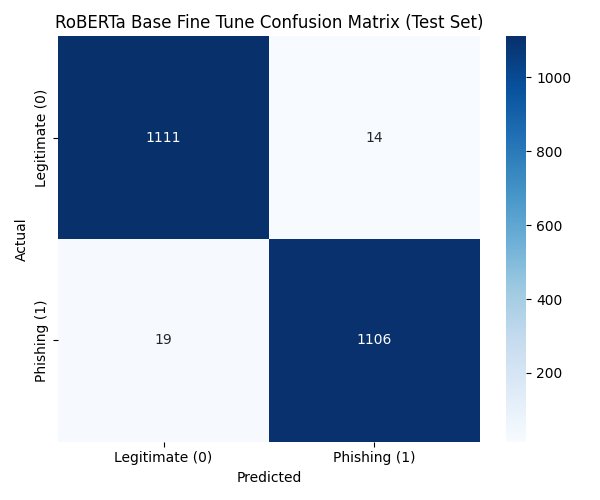
\includegraphics[width=\columnwidth]{Images/ft_roberta_base_cfm.png}
  \caption{Model 3 Confusion Matrix}
  \label{fig:model3-confmatrix}
\end{figure}

\subsection{Model 4: ELECTRA Base}
Examination of the ELECTRA model's test metrics reveals a precision of 0.9884 that is slightly higher than its recall of 0.9813, indicating that the model is marginally more conservative in its phishing classifications. As shown in Figure~\ref{fig:model4-confmatrix}, the model very rarely misclassifies a legitimate email as phishing (low false positives), which is a desirable property for practical deployment. However, the gap between precision and recall suggests that the primary source of errors is false negatives; that is, phishing emails that the model fails to flag.

This pattern is consistent with the hypothesis that ELECTRA's discriminative pretraining objective makes it highly sensitive to local lexical anomalies. As a result, phishing emails that avoid obvious structural irregularities and instead replicate the language patterns of legitimate correspondence are more likely to evade detection. For example, a qualitatively inspected test case with a high error margin (which the model confidently misclassified as legitimate) contained the following body: \textit{"Hi team, please review the updated corporate holiday schedule attached here: [URL]."} Because the text structure mimics routine administrative messaging and omits high-signal spam markers like "urgent," "password," or strange capitalization, the semantic analyzer generated a heavily skewed false-negative classification. Future work could address this by exposing the model to a wider variety of adversarial phishing examples during fine-tuning, or by combining ELECTRA's predictions with metadata-based signals such as sender domain reputation.

\begin{figure}[h]
  \centering
  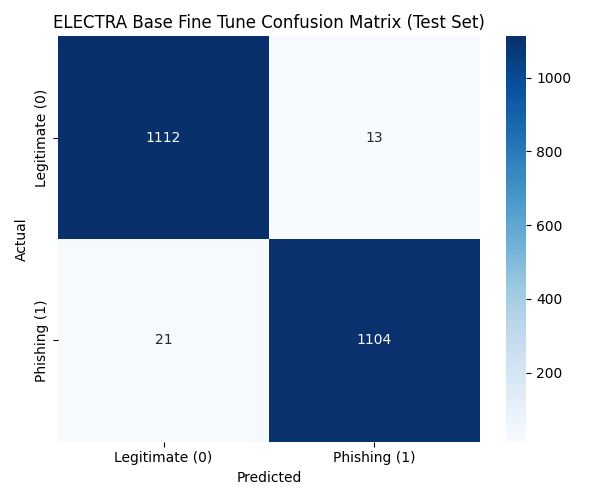
\includegraphics[width=\columnwidth]{Images/ft_electra_base_cfm.png}
  \caption{Model 4 Confusion Matrix}
  \label{fig:model4-confmatrix}
\end{figure}

\section{Conclusions}

In this project, we successfully developed and evaluated four distinct machine learning architectures for the task of phishing email detection: a hybrid Logistic Regression and RoBERTa ensemble, a Random Forest classifier utilizing TF-IDF bigrams and explicit metadata, and two standalone fine-tuned transformer models (RoBERTa-Base and ELECTRA). All implementations effortlessly surpassed the provided Codabench baselines, tightly clustering around an F1-score of 0.98. The results demonstrate that while fine-tuned contextual language models easily achieve state-of-the-art performance, traditional tree-based implementations remain highly competitive and computationally efficient when supplemented with well-engineered static features.

Despite these strong results, error analysis identified a common weakness across all four models: a shared struggle to classify deceptive threats that avoid typical spam keywords and mimic legitimate emails. These deceptive phishing emails often bypassed the classifiers, serving as the main source of false negatives. 

Moving forward, we recommend that future research looks beyond simple text representations to solve this performance limit. Future work should focus on building hybrid pipelines that use the language understanding of fine-tuned models alongside external checks, such as sender authentication and URL verification. Additionally, training the models on harder adversarial examples could further strengthen our models against methods used to hide from filters.

\section*{Team Contributions}

Hamza built Model 1 (RoBERTa and TF-IDF Ensemble) and wrote the Introduction and Related Work sections. Omar built Model 2 (Random Forest Classifier) and wrote the Dataset section. Virochaan built Model 3 (RoBERTa Base) and wrote the evaluation comparisons to other groups. Mahboob built Model 4 (ELECTRA Base), wrote the Conclusions section, and integrated the generic content formatting across the rest of the report.

% Bibliography entries for the entire Anthology, followed by custom entries
%\bibliography{custom,anthology-overleaf-1,anthology-overleaf-2}

% Custom bibliography entries only
\bibliography{custom}

% \appendix

% \section{Example Appendix}
% \label{sec:appendix}

% This is an appendix.

\end{document}
